
\documentclass[applications]{gen-bioinformatics}

\makeatletter
\renewcommand\boldmath{\@nomath\boldmath\mathversioo
n{bold}}
\makeatother

\definecolor{BiocBlue}{RGB}{24,129,194}
\usepackage{amssymb,amsfonts,url,times}
\usepackage[linkcolor=BiocBlue,pdfborder={0 0 0},urlcolor=BiocBlue]{hyperref}
\usepackage{graphics}
\usepackage{amsmath}
\usepackage{fontawesome}
\usepackage{dcolumn}
\newcolumntype{.}{D{.}{.}{-1}}
%\usepackage{hlight}

\urlstyle{rm}
\def\email#1{#1}



\newcommand{\Rfunction}[1]{{\texttt{#1}}}
\newcommand{\Robject}[1]{{\texttt{#1}}}
\newcommand{\Rpackage}[1]{{\textit{#1}}}
\newcommand{\BiocpackageFirstBAD}[1]{{\emph{\href{https://bioconductor.org/packages/3.8/#1}{#1\textsubscript{\faExternalLink}}}}} 
\newcommand{\Biocpackage}[1]{{\textit{#1}}}
\newcommand{\BiocpackageFirst}[1]{{\textit{#1}}}
\newcommand{\CRANpackage}[1]{{\emph{\href{https://cran.r-project.org/web/packages/#1/index.html}{#1}}}}
\newcommand{\CRANpackageFirst}[1]{{\emph{\href{https://cran.r-project.org/web/packages/#1/index.html}{#1}}}}
\newcommand{\CRANpackageFirstBAD}[1]{{\emph{\href{https://cran.r-project.org/web/packages/#1/index.html}{#1\textsubscript{\faExternalLink}}}}}
\newcommand{\Rmethod}[1]{{\texttt{#1}}}
\newcommand{\Rfunarg}[1]{{\texttt{#1}}}
\newcommand{\Rclass}[1]{{\texttt{#1}}}
\providecommand{\OO}[1]{\operatorname{O}\left(#1\right)}
 

\author[1]{\pfnm{Shweta}
  \pinit{}
  \psnm{Gopaulakrishnan}}

\author[1]{\pfnm{Samuela}
  \pinit{}
  \psnm{Pollack}}

\author[1]{\pfnm{Benjamin}
  \pinit{}
  \psnm{Stubbs}}

\author[2]{\pfnm{Herv\'e}
  \pinit{}
  \psnm{Pag\`es}}

\author[3]{\pfnm{John}
  \pinit{}
  \psnm{Readey}}

\author[4]{\pfnm{Sean}
  \pinit{}
  \psnm{Davis}}

\author[5]{\pfnm{Levi}
  \pinit{}
  \psnm{Waldron}}

\author[6]{\pfnm{Martin}
  \pinit{T}
  \psnm{Morgan}}

\author[1]{\pfnm{Vincent}
  \pinit{J}
  \psnm{Carey}}

\address[1]{\porgdiv{Channing Division of Network Medicine}
  \porgname{Brigham and Women's Hospital}
  \pstreet{181 Longwood Avenue }
  \pcity{Boston}
  \postcode{02115}
  \pcnty{USA}}

\address[2]{\porgdiv{Systems Bioinformatics}
  \porgname{Fred Hutchinson Cancer Research Center}
  \pstreet{Fairview Avenue }
  \pcity{Seattle}
%  \postcode{}
  \pcnty{USA}}

\address[3]{
  \porgname{HDF Group}
%  \pstreet{}
  \pcity{Seattle}
%  \postcode{}
  \pcnty{USA}}

\address[4]{\porgdiv{Center for Cancer Research}
  \porgname{NCI}
  \pcity{Bethesda}
  \pcnty{USA}}


\address[5]{
  \porgdiv{Institute for Implementation Science in Population Health}
  \porgname{CUNY School of Public Health}
  \pcity{NY}
  \pcnty{USA}}

\address[6]{
  \porgname{RPCI}
%  \pstreet{}
  \pcity{Buffalo}
%  \postcode{}
  \pcnty{USA}}

\hyphenation{Sum-mar-ized-Exp-er-i-ment} 
\hyphenation{hsds-hdf-lab}
\hyphenation{hdf-group}

\begin{document}


\title{Supplemental material for 'restfulSE: a semantically rich interface for cloud-scale genomics
with Bioconductor'}
\maketitle

\begin{abstract}
\begin{subabstract}[Summary]
Clients for
HDF5 (\url{https://www.hdfgroup.org/}) or BigQuery (\url{https://cloud.google.com/bigquery/}) are available in numerous languages.
The
Bioconductor interfaces described here and
in the main paper support access to archives of genomic
data resident in these "bigdata back ends". 
Our intent is to allow the
use of familiar and semantically meaningful programmatic idioms
to query genomic data,
while abstracting the remote interface from end users
and developers.
This document provides installation details and extended
analysis and performance considerations for the main paper.
\end{subabstract}
\begin{subabstract}[Availability] Packages \BiocpackageFirst{restfulSE} and
\BiocpackageFirst{BiocOncoTK} of Bioconductor
 (\url {bioconductor.org}).  Artistic-2.0 licensing.  
\end{subabstract}
\begin{subabstract}[Contact]reshg@channing.harvard.edu
\end{subabstract}
%\begin{subabstract}[keywords] REST API, HDF5, Bioconductor
\end{abstract}

\section*{Setup}
\subsection*{Installation}

Programming detailed in the main paper requires 
version 3.5 (or later) of R.  With this version
of R, package installation occurs using the
BiocManager package, available at cran.r-project.org.

Code described in the main paper and supplement can be 
executed after the following commands succeed:
\begin{verbatim}
library(BiocManager)
install(version = "devel")
install(c("restfulSE", "BiocOncoTK",
   "rhdf5client"))
\end{verbatim}
The \texttt{install} command will install additional
required packages to establish a suitable environment
for the examples to run.

\subsection*{Authentication for Google BigQuery}

A Google Cloud Platform Project ID is needed to
permit use of BigQuery.  This can be established \textit{de novo}
by running \textit{gcloud auth login}, selecting a Google
identity, and establishing the name of a project for
the BigQuery app.  Browse to \texttt{console.cloud.google.com/bigquery}
and find the current Project ID or create a new one.

The ID should be supplied to \verb+pancan_BQ+ as the
\texttt{billing} parameter to establish the BigQueryConnection
instance for R.  The ID can also be used as the setting
of the environment variable \verb+CGC_BILLING+, which
\verb+pancan_BQ+ will use as billing parameter if none
is supplied in a call.


\section*{Data structures for remote back ends}

\subsection*{The \texttt{SummarizedExperiment} class and related methods}

Let $Q$ denote a matrix of quantifications arising from a genome
scale assay with $G$ assay features measured on $N$ experimental
samples.  The elements of $Q$ are the numbers $q_{ij}, i = 1, \ldots, G,
j = 1, \ldots, N$.  Bioconductor's \texttt{SummarizedExperiment} structure
manages feature quantifications
with associated metadata about assay features
and samples.

In the 10x mouse neuron dataset, $G=27998$ and $N=1.3$ million.
When these quantifications are managed in a Bioconductor \texttt{SummarizedExperiment X}, the matrix $Q$ is programmatically bound to a $G \times F$
table of feature-level metadata (e.g., gene or transcript names and
characteristics) accessible by the \texttt{rowData} method, and to an $N \times R$ table of sample-level metadata accessible by \texttt{colData} \citep{Huber2015}. 
The standard subsetting idiom \texttt{X[G,S]} expresses filtering of 
the all the information in $Q$ and the associated metadata
to features \texttt{G} and samples \texttt{S}.  A \texttt{GRanges} 
instance \citep{Lawrence2013} defining genomic coordinates for features may be bound to \texttt{X},
facilitating queries defined by genomic location (using, for example, \texttt{subsetByOverlaps}) to isolate features
coincident with or near the elements of a set of query genomic ranges (eg., binding peaks).  This outline of genomic data representation
and analysis is characteristic of Bioconductor.

\subsection*{Current remote back ends}

\textit{Google BigQuery.} The Institute for Systems Biology Cancer
Genomics Cloud project (ISB-CGC) \citep{ISBCGC} uses 
Google BigQuery to provide access to
various public cancer genomics resources including
TCGA and the PanCancer Atlas \citep{Hoadley2018}.
The \verb+pancan_SE+
function of \Biocpackage{restfulSE} constructs queries that derive
\texttt{SummarizedExperiment} instances using quantifications and annotations
for PanCancer atlas experiments
managed in BigQuery tables.  

\noindent
\textit{HDF Scalable Data Service (HSDS).}
An AWS S3-based distributed data object model for
HDF5 datasets, including a
RESTful API to structure, populate, and query HDF5 archives, 
has been implemented by the HDF Group. 
A number of datasets of interest in bioinformatics
are served through \url{https://www.hdfgroup.org/solutions/hdf-kita/}
in the \texttt{/shared/bioconductor} folder.

\subsection*{Lazy data retrieval via DelayedArray.}

The \Biocpackage{restfulSE} package provides interfaces to 
BigQuery and HSDS so that 
the numerical content housed in these services
satisfies the API of the Bioconductor \BiocpackageFirst{DelayedArray} package \citep{Pages2018}.  
Any \verb+DelayedArray+ instance can serve as the \verb+assay+
component of a \texttt{SummarizedExperiment} instance.  Thus the
capacities of \verb+SummarizedExperiment+ to bind semantically
rich metadata to genome-scale assays are extended implicitly to
data resources for which no standards exist for
associating substantive metadata.  
In conjunction with the \BiocpackageFirst{rhdf5client} \citep{rclient} and \CRANpackageFirst{bigrquery} \citep{bigr} packages,
\Biocpackage{restfulSE} translates filtering and selection operations
which are readily defined using \verb+rowData+, \verb+rowRanges+,
and \verb+colData+ into formal queries resolvable by the HDF5 and
BigQuery services.  Numerical results are transmitted from
server to client only when needed.

\section*{Extended examples}

The RESTful \texttt{SummarizedExperiment} representation
allows complicated research queries to be obtained in a concise,
fast, convenient and robust fashion, as illustrated by
the following examples.


\subsection*{Multitumor, multigene survey of association
of gene expression with microsatellite instability}

Figure \ref{pancanPanel} illustrates the 
use of the \Biocpackage{restfulSE} protocol
with the ISB-CGC BigQuery back end.  Figure 5C
of \citet{Bailey2018} indicates that
microsatellite instability (MSI) is associated with
different expression signatures of immune cell infiltration
for adenocarcinomas of colon (COAD) and stomach (STAD), and
uterine corpus endometrial carcinoma (UCEC).  
The MSI scores developed using MSIsensor are found
in Table S5 of \cite{Ding2018}.
Code at the top of Figure \ref{pancanPanel} employs
functions in the \BiocpackageFirst{BiocOncoTK} \citep{bionc} package that build on
\Biocpackage{restfulSE} functionality to a) authenticate the
user to the BigQuery platform, b) select a tumor
type (COAD) and assay for \texttt{SummarizedExperiment}
construction, c) bind Ding et al.'s MSI values as
sample-level data variable \verb+msiTest+, d)
acquire and transform the PD-L1 
(Entrez ID 29126)
expression values, and e) form the stratified boxplot. 
The basic findings of Bailey et al. are replicated.
Enhancement of the code to produce the 3 x 3 tableau
is demonstrated in the \Biocpackage{BiocOncoTK} \citep{bionc} vignette.
Note that in this example, expression values are
only downloaded for a single gene, without altering
the end user programming paradigm.

\begin{figure}
\begin{verbatim}
library(SummarizedExperiment)
library(BiocOncoTK) # uses restfulSE
bq = pancan_BQ() # need CGC_BILLING
seCOAD = bindMSI(buildPancanSE(bq, 
  acronym="COAD", assay="RNASeqv2"))
boxplot(split(log2(as.numeric(assay(
 seCOAD["29126",]))+1), 
      seCOAD$msiTest >= 4),
      names = c("<4", ">=4"), 
      ylab="PD-L1")
\end{verbatim}
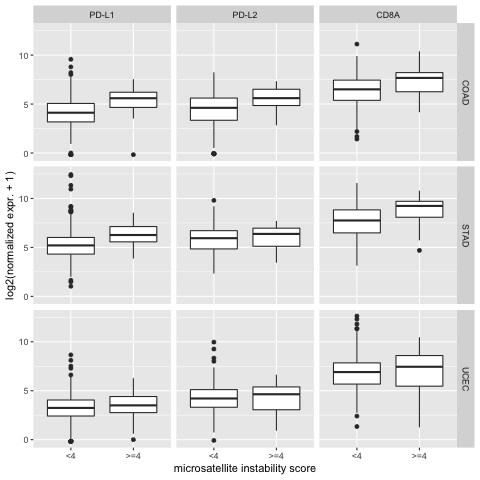
\includegraphics[height=8.0cm]{microsatpan2.png}
\caption{Top: Code for base graphics display of boxplot
corresponding to top left panel of lower display.
Bottom: Reassessment of immune infiltrate expression
patterns stratified by microsatellite instability
status and tumor type, as reported in \cite{Bailey2018}.
Figure \ref{compl} provides all
code needed to produce the nine panel display.}
\label{pancanPanel}
\end{figure}



\subsection*{Comparing cell-type-specific 
expression distributions after immunopanning}

Figure \ref{hdffig}
demonstrates use of a RESTful SummarizedExperiment,
with assay data \texttt{/shared/biocond- uctor/darmgcls.h5}
at hsdshdflab.hdfgroup.org.  Briefly, as a
prelude to single-cell RNA-sequencing of glioblastoma (GBM)
tumors from four patients,
\cite{Darmanis2017} used immunopanning to increase the
proportion of non-neoplastic cells that constitute
the "migrating front" of progression of glioblastoma.
Antibody to CD45 was used to capture microglial cells.
Figure \ref{hdffig} provides code to compare
the distribution of CD45 expression among the
classes of
cells as labeled in the metadata of GSE84465,
the NCBI GEO archive from which the quantifications
were derived.  
In this example, data on one
gene from all cells
is retrieved when the statement defining vector \texttt{vals}
is executed.  The display can be recapitulated for
other genes by substituting different symbols in
the statement computing \texttt{ind}.
The \verb+DelayedArray+ framework leveraged here
enables basic computations of this kind without loading the
entire matrix into memory.


\begin{figure}
\begin{verbatim}
library(rhdf5client)
library(SummarizedExperiment)
library(BiocOncoTK)
library(ggplot2)
cdar = BiocOncoTK::darmGBMcls
ind = match("PTPRC", rowData(cdar)$symbol)
var = gsub("selection: ", "", 
       cdar$characteristics_ch1.8)
vals = log10(assay(cdar[ind,])+1)
ddd = data.frame(log10norm=vals, pan=var)
ggplot(ddd, aes(x=log10norm, colour=pan)) + 
  geom_density() + ylim(0,1) + 
  xlab("log10 CD45+1")
\end{verbatim}
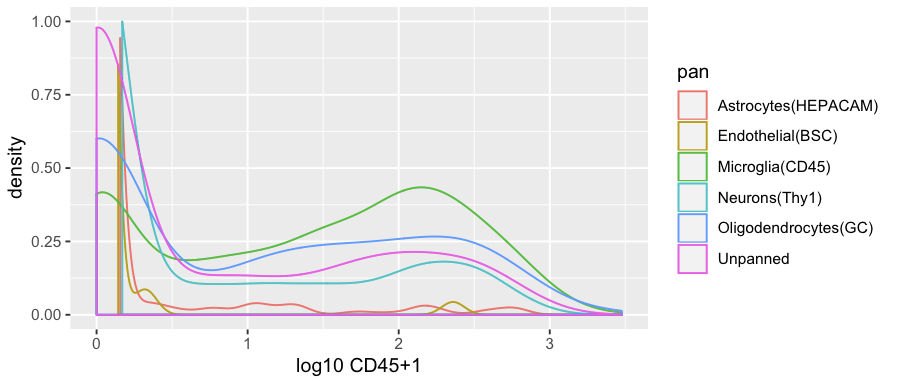
\includegraphics[height=4.0cm]{darmDens.png}
\caption{Code and density displays for
distribution of PTPRC (HGNC symbol for CD45) across immunopanned
cells reported in \cite{Darmanis2017}.
\texttt{BiocOncoTK::darmGBMcls} includes
a reference to HDF Cloud representation of
this glioblastoma single-cell RNA-seq
as requantified in the CONQUER project \citep{Soneson2018}.}
\label{hdffig}
\end{figure}



\noindent
%\textbf{HDF Cloud back end.}  Figure \ref{hdffig}
%demonstrates construction of a RESTful \texttt{SummarizedExperiment}
%for expression data on 1.3 million neurons.
%The syntax \verb+tenx[,s]+ generates a delayed selection for
%all genes with samples 
%identified in vector \verb+s+.  Invoking the \verb+assay()+
%method triggers RESTful queries to the object store at \verb+URL_hsds()+.
%These can be serviced in parallel, with
%throughput dependent on the configuration
%of the HSDS server and its load at time of request.
%Replies can be requested in JSON or binary formats;
%\Rpackage{rhdf5client} utilities handle parsing the
%responses into R matrix structures.
%In this example, data for only four of 1.3 million neurons
%are downloaded and used to compute sums of RNA-seq read
%counts.  The \verb+DelayedArray+ framework leveraged here
%enables basic computations of this kind without loading the
%entire matrix into memory.



\section*{Performance}

We focus on pursuit of reliability,
expressivity, and scalability using \Biocpackage{restfulSE}.  
\textit{Reliability:} 
The \Biocpackage{restfulSE}, \Biocpackage{rhdf5client} \citep{rclient},
and \Biocpackage{BiocOncoTK} \citep{bionc} packages are accompanied by detailed unit
tests that compare retrievals to known values.  In the
case of BigQuery table queries, the test
suite composes random queries 
in both BigQuery SQL and in the \texttt{SummarizedExperiment} 
idiom.  Results
are checked for elementwise equality.  \textit{Expressivity:} The code
segments in Figures \ref{pancanPanel} and \ref{hdffig} are
complex but easy to break down.  The joining and
reshaping of pancan-atlas tables in BigQuery corresponding
to the code in Figure \ref{pancanPanel}
can be checked through the query history in the BigQuery
interface.  The acquisition of expression values required
five nested SELECT statements; the query for assay quantifications
was 6000 characters in length.
The R code is 223 characters including comments.
\textit{Scalability.}  BigQuery is intrinsically auto-scaling,
but charges accrue with the amount of data scanned, 
so query design can have effects on throughput
and cost.  We rely on the \CRANpackage{bigrquery} \citep{bigr} and \CRANpackageFirst{dbplyr} \citep{dbp} packages for
efficient translation of R-oriented data manipulations to 
BigQuery SQL.  Throughput with HDF Cloud 
is dependent upon the configuration of the object server,
the relationship of numerical data layout to prevalent access
patterns, and the degree to which queries capitalize on
API efficiencies like chunk-based retrieval.  For both
back ends, proper design and deployment of the querying client can
lead to throughput that scale with client-side resources.

\section*{Conclusions}

Cloud-scale storage and retrieval strategies are of significant
interest for genome science.  
The \Rclass{SummarizedExperiment} class
unifies assay data with substantive sample- and experiment-level
metadata, and its API for managing and interrogating
genome-scale experiment archives is used in numerous
analytic packages.  
The \Biocpackage{restfulSE} package exposes high-performance
cloud-resident data stores to users and
algorithms as \texttt{SummarizedExperiment}+s.  Continued improvements
in efficiency of
representation and query resolution for assay data and metadata
will help to achieve the potential of a federated data ecosystem for
enhanced discovery in biology through interactive genome-scale analysis.


\begin{figure}
{\small
\begin{verbatim}
library(BiocOncoTK)
# set up gene x tumor table
infilGenes = c("CD274", 
  "PDCD1LG2", "CD8A")
names(infilGenes) = c("PD-L1", "PD-L2", 
   "CD8A")
tumcodes = c("COAD", "STAD", "UCEC")
combs = expand.grid(tumcode=tumcodes, 
  ali=names(infilGenes),
    stringsAsFactors=FALSE)
combs$sym = infilGenes[combs$ali]

# establish BigQueryConnection
bq = pancan_BQ() #billing=[project id])

# build a data.frame for ggplot, using
# bindMSI to add microsatellite instability 
# scores  and replaceRownames to convert 
# ENTREZ ids (used
# natively in ISB BigQuery 
# pancan-atlas) to HGNC symbols
exprByMSI = function(bq, tumcode, genesym, 
    alias) {
  if (missing(alias)) alias=genesym
  ex = bindMSI(buildPancanSE(bq, tumcode, 
    assay="RNASeqv2"))
  ex = replaceRownames(ex)
  data.frame(
   patient_barcode=colnames(ex),
   acronym=tumcode,
   symbol = genesym,
   alias = alias,
   log2ex=log2(
     as.numeric(
      SummarizedExperiment::assay(
       ex[genesym,]))+1),
   msicode = ifelse(ex$msiTest >= 4, 
      ">=4", "<4"))
 }

# apply exprByMSI to each tumor
updateL = lapply(1:nrow(combs), function(x) 
   exprByMSI(bq, combs$tumcode[x], 
     combs$sym[x], combs$ali[x]))
updated = do.call(rbind, updateL)
# visualize
library(ggplot2)
ggplot(updated,
    aes(msicode, log2ex)) + geom_boxplot() +
    facet_grid(acronym~alias) +
    ylab("log2(normalized expr. + 1)") +
    xlab("microsatellite instability score")
\end{verbatim}
}
\label{compl}
\caption{Complete code to compute the panel of Figure \ref{pancanPanel}.}
\end{figure}


\section*{Acknowledgments}
Support for the development of this software was provided by NIH grants
U01 CA214846 (Carey, PI) and U24 CA180996 (Morgan, PI).

\bibliography{BioC}

\end{document}
